% !Mode:: "TeX:UTF-8"
\documentclass{article}
% !Mode:: "TeX:UTF-8"
\usepackage[english]{babel}
\usepackage[UTF8]{ctex}
\usepackage{amsmath, amsthm, amssymb}

% Figure
\usepackage{graphicx}
\usepackage{float} %% H can fix the location
\usepackage{caption}
\usepackage[format=hang,singlelinecheck=0,font={sf,small},labelfont=bf]{subfig}
\usepackage[noabbrev]{cleveref}
\captionsetup[subfigure]{subrefformat=simple,labelformat=simple,listofformat=subsimple}
\renewcommand\thesubfigure{(\alph{subfigure})}

\usepackage{epstopdf} %% convert eps to pdf
\DeclareGraphicsExtensions{.eps,.mps,.pdf,.jpg,.png} %% bmp, gif not supported
\DeclareGraphicsRule{*}{eps}{*}{}
\graphicspath{{img/}{figure/}{../figure/}} %% fig directorys

%% \usepackage{pstricks} %% a set of macros that allow the inclusion of PostScript drawings directly inside TeX or LaTeX code
%% \usepackage{wrapfig} %% Wrapping text around figures

% Table
\usepackage{booktabs} %% allow the use of \toprule, \midrule, and \bottomrule
\usepackage{tabularx}
\usepackage{multirow}
\usepackage{colortbl}
\usepackage{longtable}
\usepackage{supertabular}

\usepackage[colorinlistoftodos]{todonotes}

% Geometry
\usepackage[paper=a4paper, top=1.5cm, bottom=1.5cm, left=1cm, right=1cm]{geometry}
%% \usepackage[paper=a4paper, top=2.54cm, bottom=2.54cm, left=3.18cm, right=3.18cm]{geometry} %% ms word
%% \usepackage[top=0.1cm, bottom=0.1cm, left=0.1cm, right=0.1cm, paperwidth=9cm, paperheight=11.7cm]{geometry} %% kindle

% Code
%% \usepackage{alltt} %% \textbf can be used in alltt, but not in verbatim

\usepackage{listings}
\lstset{
    backgroundcolor=\color{white},
    columns=flexible,
    breakatwhitespace=false,
    breaklines=true,
    captionpos=tt,
    frame=single, %% Frame: show a box around, possible values are: none|leftline|topline|bottomline|lines|single|shadowbox
    numbers=left, %% possible values are: left, right, none
    numbersep=5pt,
    showspaces=false,
    showstringspaces=false,
    showtabs=false,
    stepnumber=1, %% interval of lines to display the line number
    rulecolor=\color{black},
    tabsize=2,
    texcl=true,
    title=\lstname,
    escapeinside={\%*}{*)},
    extendedchars=false,
    mathescape=true,
    xleftmargin=3em,
    xrightmargin=3em,
    numberstyle=\color{gray},
    keywordstyle=\color{blue},
    commentstyle=\color{green},
    stringstyle=\color{red},
}

% Reference
%% \bibliographystyle{plain} % reference style

% Color
\usepackage[colorlinks, linkcolor=blue, anchorcolor=red, citecolor=green, CJKbookmarks=true]{hyperref}
\usepackage{color}
\def\red#1{\textcolor[rgb]{1.00,0.00,0.00}{#1}}
\newcommand\warning[1]{\red{#1}}

% Other
%% \usepackage{fixltx2e} %% for use of \textsubscript
%% \usepackage{dirtree}  %% directory structure, like the result of command tree in bash shell


% !Mode:: "TeX:UTF-8"
%+++++++++++++++++++++++++++++++++++article+++++++++++++++++++++++++++++++++
%customize the numbering of equation, to make it like section-subsection-equation style, for example,1-2-3
\makeatletter\@addtoreset{equation}{subsection}\makeatother
\renewcommand\theequation{%
\thepart\arabic{section}%
-\thepart\arabic{subsection}%
-\thepart\arabic{equation}%
}
%theorem
\newtheorem{definition}{D\'efintion} %% 整篇文章的全局编号
\newtheorem*{thmwn}{Thm} %% without numbers
\newtheorem{theorem}{Th\'eor\`eme}[section] %% 从属于section编号
\newtheorem{corollary}{Corollary}[theorem] %% 从属于theorem编号
\newtheorem{lemma}{Lemma}
\newtheorem{proposition}{Proposition}[section]
\newtheorem{example}{Example}
\newtheorem*{attention}{Attention}
\newtheorem*{note}{Note}
\newtheorem*{remark}{Remark}
\newtheorem{question}{Question}[section]
\newtheorem{problem}{Problem}
\newtheorem{fact}{Fact}


% Equation
\newcommand\lasteq{(\theequation)\ } %% use \lasteq to reference the last equation
\newcommand{\eqspace}{\hspace{0.5cm}}
\newcommand{\eqnote}[1]{\text{ #1 }} %% insert text in math mode being treated as normal text
\newcommand\mytop[2]{\genfrac{}{}{0pt}{}{#1}{#2}} %% generate a fraction but without the line

% Vecteur
\def\vecteur#1{(#1_1,~#1_2,~\ldots,~#1_n)}
\def\vector#1{#1_1,~#1_2,~\ldots,~#1_n}

% Set
\newcommand{\R}{\mathbb{R}} %% the real number set
\newcommand{\N}{\mathbb{N}}
\newcommand{\Z}{\mathbb{Z}}
\newcommand{\Q}{\mathbb{Q}}
\newcommand{\set}[1]{\{#1\}}
\newcommand{\stcomp}[1]{\overline{#1}} %% set complement

% Logic
\newcommand{\si}{\textrm{\ if }}
\newcommand{\sinon}{\textrm{ si non}}
\newcommand{\then}{\textrm{ then }}
\newcommand{\et}{\textrm{\ et }}
\newcommand{\ou}{\textrm{ ou }}
\newcommand{\non}{\textrm{non }}
\newcommand{\ssi}{si et seulement si }

% Math Operator
\newcommand{\fun}[1]{\textit{#1}}
\DeclareMathOperator{\arccot}{arcot}
\DeclareMathOperator{\arcth}{arcth}
\DeclareMathOperator{\arcsh}{arcsh}
\DeclareMathOperator{\arch}{arch}
\DeclareMathOperator{\ch}{ch}
\DeclareMathOperator{\dth}{th} %% \th already used
\DeclareMathOperator{\sh}{sh}
\DeclareMathOperator{\var}{var}
\DeclareMathOperator{\Ker}{Ker}
\DeclareMathOperator{\Img}{Img}

\newcommand*\laplace{\mathop{}\!\mathbin\bigtriangleup}
\newcommand*\dalambert{\mathop{}\!\mathbin\Box}
\newcommand{\grad}[1]{\nabla #1}
\newcommand{\gradien}[1]{\nabla #1}
\newcommand{\divergence}[1]{\nabla \cdot #1}
\newcommand{\rotationnel}[1]{\nabla \times #1}
\newcommand{\rot}[1]{\nabla \times #1}

\newcommand{\diag}[1]{\textit{diag}(#1)}
\newcommand{\mean}[1]{\overline{#1}}
\newcommand{\estimate}[1]{\hat{#1}}
\newcommand{\indep}{\!\perp\!\!\!\perp}
\newcommand{\nindep}{\not\!\perp\!\!\!\perp}
\newcommand{\norm}[1]{\left\Vert #1\right\Vert}
\newcommand{\obey}[1]{\thicksim{#1}}

\usepackage{xspace}
\newcommand{\ps}[2]{\ensuremath{\langle #1 , #2\rangle}\xspace} %% produit scalaire

%% quantique operators
\newcommand\ket[1]{|#1\rangle}
\newcommand\bra[1]{\langle #1|}
\newcommand\braket[3]{\langle#1|#2|#3\rangle}

% Symbol
\newcommand{\infinity}{\infty}


\begin{document}
\title{Optimisation}
\author{Common}
\maketitle
\newpage
\tableofcontents
\newpage

\section{线性规划的对偶问题}
\href{http://course.cug.edu.cn/cugFirst/operational\_research/main/charpter2/p1.htm}{对偶}

\subsection{对偶的引出}
假设某厂计划生产甲,乙两种产品,其主要原材料有钢材3600kg,铜材2000kg及专用设备能力3000台时,已原材料和设备的单间消耗定额以及单位产品所获利润如下表所示\href{http://course.cug.edu.cn/cugFirst/operational\_research/main/charpter1/p1.files/image001.gif}{表1-1}
问如何安排生产方使该厂所获利润最大?

为了求解这一问题,设甲,乙两种产品的计划产量分别为$x_1, x_2$件.

这个问题的数学形式表达为
\begin{equation}
max\ z = 70x_1 + 120x_2
\mbox{ subject to }
\left\{
  \begin{array}{ll}
		 9x_1 + 4 x_2 \leq 3600; \\
		 4x_1 + 5 x_2 \leq 2000; \\
		 3x_1 + 54 x_2 \leq 3000; \\
		 x_1 \geq 0, x_2 \geq 0,
  \end{array}
\right.
\label{dual.original}
\end{equation}

现在,从另一个角度来考虑该问题,假设这家企业想将自己的原材料生产产品然后卖成品\textbf{改为直接卖原材料},
此时,工厂决策者必须考虑怎样为这三种资源定价的问题.
设$y_1, y_2, y_3$分别代表转让两种资源和出租设备的价格和租金.

定价的原则是:\textbf{直接卖原材料的获利不能低于卖成品}.\\
生产一个单位的甲产品需消耗9个单位的钢材,4个单位的铜材,3个单位的设备台时,获利70个单位,
那么,将这些资源全部转让时所获得的利润应不少于70个单位,即$9y_1 + 4y_2 + 3y_3 \geq 70$\\
同样的分析,有$4y_1 + 5y_2 + 10y_3 \geq 120$\\
此时,企业的总获利(即对方的总付出)为$W = 3600y_1 + 2000y_2 + 300y_3$

\textbf{为使对方容易接受},该厂只能在上面的两个约束条件下求$W$的最小值,即
\begin{equation}
min\ W = 3600y_1 + 2000y_2 + 300y_3
\mbox{ subject to }
\left\{
  \begin{array}{ll}
		9y_1 + 4y_2 + 3y_3 \geq 70 \\
		4y_1 + 5y_2 + 10y_3 \geq 120 \\
		y_1 \geq 0, y_2 \geq 0, y_3 \geq 0,
  \end{array}
\right.
\label{dual.dual}
\end{equation}

上述两个模型\eqref{dual.original}和\eqref{dual.dual}是对同一问题的两种不同考虑的数学描述,其间有着一定的内在联系,
我们对此进行比较分析,并从中找出规律,两个模型的对应关系有:
\begin{enumerate}
\item 两个问题的系数矩阵互为转置,
\item 一个问题的变量个数等于另一个问题的约束条件个数,
\item 一个问题的右端系数是另一个问题的目标函数的系数,
\item 一个问题的目标函数为极大化,约束条件为"$\leq$"类型,另一个问题的目标函数为极小化,约束条件为"$\geq$"
\end{enumerate}
我们把这种对应关系称为对偶关系,如果把式\eqref{dual.original}称为原问题,则式\eqref{dual.dual}称为对偶问题.

\subsection{Theory}
原问题与对偶问题在某种意义上来说,实质上是一样的,因为第二个问题仅仅在第一个问题的另一种表达而已

对偶问题的对偶是原问题

\subsubsection{对称}
当原问题对偶问题只含有不等式约束时,称为对称形式的对偶, 上面的形式即为对称的

原问题
\begin{equation}
max\ z = \ps{C}{X}
\mbox{ subject to }
\left\{
  \begin{array}{ll}
	  A \cdot X \leq b \\
		X \geq 0
  \end{array}
\right.
\label{dual.model.ori}
\end{equation}

对偶问题
\begin{equation}
min\ w = \ps{b}{Y}
\mbox{ subject to }
\left\{
  \begin{array}{ll}
		A^t \cdot Y \geq C \\
		Y \geq 0
  \end{array}
\right.
\label{dual.model.dual}
\end{equation}

当原问题为3个约束, 两个变量时:
$$X=(x_1, x_2)^t$$
$$A = A_{3 \times 2},\ A^t = A^t_{2 \times 3}$$
$$b = (b_1, b_2, b_3)^t$$
$$Y = (b_1, b_2, b_3)^t$$
$$C=(c_1, c_2)^t$$

\subsubsection{非对称}
若原问题的约束条件是等式, 称为非对称形式的对偶

原问题
\begin{equation}
max\ z = \ps{C}{X}
\mbox{ subject to }
\left\{
  \begin{array}{ll}
	  A \cdot X = b \\
		X \geq 0
  \end{array}
\right.
\end{equation}

对偶问题
\begin{equation}
min\ w = \ps{b}{Y}
\mbox{ subject to }
\left\{
  \begin{array}{ll}
		A^t \cdot Y \geq C \\
		Y \mbox{无约束}
  \end{array}
\right.
\end{equation}

\begin{proof}
$$
\mbox{原问题}
\Leftrightarrow
\left\{
  \begin{array}{ll}
	max\ z = \ps{C}{X} \\
	  A \cdot X \geq b \\
	  A \cdot X \leq b \\
		X \geq 0
  \end{array}
\right.
\Rightarrow
\left\{
  \begin{array}{ll}
	max\ z = \ps{C}{X} \\

    \begin{bmatrix}
        A \\
        -A \\
    \end{bmatrix}

    X \leq

    \begin{bmatrix}
        b \\
        -b \\
    \end{bmatrix} \\

		X \geq 0
  \end{array}
\right.
$$

根据对称形式的对偶模型,可直接写出上述问题的对偶问题
$$
\Rightarrow
\left\{
  \begin{array}{ll}
	min\ w = \ps{
    \begin{bmatrix}
        b \\
        -b \\
    \end{bmatrix}
	}{Y} \\

    \begin{bmatrix}
        A \\
        -A \\
    \end{bmatrix}^t

    Y \geq C \\

		Y \geq 0
  \end{array}
\right.
$$

$$
\mbox{设 }
Y =
    \begin{bmatrix}
        Y_1 \\
        Y_2 \\
    \end{bmatrix}
$$

$$
\Rightarrow
\left\{
  \begin{array}{ll}
	min\ w = \ps{b}{Y_1 - Y_2} \\
	A(Y_1 - Y_2) \geq C \\
	Y_1, Y_2 \geq 0
  \end{array}
\right.
$$
再令$Y = Y_1 - Y_2$(这个新的$Y$和之前的$Y$不同), 得到对偶问题为:
$$
\left\{
  \begin{array}{ll}
	min\ w = \ps{b}{Y} \\
	A(Y) \geq C \\
	Y \mbox{无约束}
  \end{array}
\right.
$$
\end{proof}

\subsubsection{Theorem}
\begin{theorem}
\textbf{弱对偶性定理}
若$\overline{X}$ 和 $\overline{Y}$ 分别是原问题\eqref{dual.model.ori}及对偶问题\eqref{dual.model.dual}的可行解,则有
$$ \ps{C}{\overline{X}} \leq \ps{b}{\overline{Y}} $$
\end{theorem}
\begin{proof}
$$
\left\{
  \begin{array}{l}
	  A \cdot \overline{X} \leq b \Rightarrow \overline{Y}^t \cdot A \cdot \overline{X} \leq \overline{Y}^t \cdot b \Rightarrow \ps{A\overline{X}}{\overline{Y}} \leq \ps{b}{\overline{Y}} \\
	  A^t \cdot \overline{Y} \geq C \Rightarrow \overline{X}^t \cdot A^t \cdot \overline{Y} \geq \overline{X}^t \cdot C \Rightarrow \ps{A\overline{X}}{\overline{Y}} \geq \ps{C}{\overline{X}}
  \end{array}
\right.
\Rightarrow
\ps{C}{\overline{X}} \leq \ps{b}{\overline{Y}}
$$
\end{proof}

从弱对偶性可得到以下重要结论:
\begin{enumerate}
\item 极大化问题(原问题)的任一可行解所对应的目标函数值是对偶问题最优目标函数值的下界.
\item 极小化问题(对偶问题)的任一可行解所对应的目标函数值是原问题最优目标函数值的上界.
\item 若原问题可行,但其目标函数值无界,则对偶问题无可行解.
\item 若对偶问题可行,但其目标函数值无界,则原问题无可行解.
\item 若原问题有可行解而其对偶问题无可行解,则原问题目标函数值无界.
\item 对偶问题有可行解而其原问题无可行解,则对偶问题的目标函数值无界.
\end{enumerate}

\begin{theorem}
\textbf{最优性定理}:
若$X^*$ 和 $Y^*$ 分别是原问题\eqref{dual.model.ori}及对偶问题\eqref{dual.model.dual}的可行解,且有$\ps{C}{X^*} = \ps{b}{Y^*}$,
则$X^*,Y^*$分别是\eqref{dual.model.ori}和\eqref{dual.model.dual}的最优解.
\end{theorem}

\begin{theorem}
\textbf{强对偶定理}:
若原问题及其对偶问题均具有可行解,则两者均具有最优解,且它们最优解的目标函数值相等.
\end{theorem}
\begin{proof}
原问题与对偶问题的解一般有三种情况:
\begin{enumerate}
\item 一个有有限最优解 $\Rightarrow$ 另一个有有限最优解.
\item 一个有无界解 $\Rightarrow$ 另一个无可行解.
\item 两个均无可行解.
\end{enumerate}
\end{proof}

\begin{theorem}
\textbf{(对偶定理}:
若线性规划问题\eqref{dual.model.ori}和\eqref{dual.model.dual}之一有最优解,则另一问题也有最优解,并且两者的目标函数值是相等的
\end{theorem}

\subsection{对偶问题的经济解释}
\href{http://course.cug.edu.cn/cugFirst/operational\_research/main/charpter2/p4.htm}{demo}

对于线性规划问题\eqref{dual.model.ori},用它来处理资源分配问题时,其决策变量代表的是产品的产量.它的对偶问题\eqref{dual.model.dual},其对偶变量也有明显的经济意义.
事实上,若$X^* = (x^*_1, x^*_2, \ldots, x^*_n)^t$
为原问题\eqref{dual.model.ori}的最优解,最优目标函数值为$z^*$.根据对偶定理,对偶问题也有最优解$Y^* = (y^*_1, y^*_2, \ldots, y^*_n)^t$.
且两者的最优目标函数值相等,即:
$$z^* = \ps{C}{X^*} = \ps{b}{Y^*} = w^*$$,
 
这也就是说,原问题的目标函数值等于$\sum_i b_i y^*_i$.由于这个和为各个$b_i y^*_i$相加而成,故可以将每个$b_i y^*_i$ 看成是第i种资源对目标函数值所做的贡献.
又由于 $b_i$ 是第i种资源的拥有量,因此, $\dfrac{b_i y^*_i}{b_i} = y^*_i$ 便可以理解为是每个单位第i种资源对目标函数值的贡献.
即:增加或减少单位第i种资源所引起总收益(目标函数)的改变量.

我们称 $y^*_i$ 为第i种资源的\textbf{影子价格}.显然这种价格不同于第i种资源的市场价格,它是由企业内部的条件决定的.\\
影子价格是一种边际价格, $\dfrac{\partial z^*}{b_i} = y^*_i$

同一种资源在不同的企业影子价格一般可以不同.一种资源的影子价格越大,则增加或减少一个单位这种资源,对总收益的影响越大,
如果一种资源的影子价格为零,则在一定范围内增加或减少一个单位这种资源对总收益没有影响.

\section{拉格朗日乘数}
微积分中最常见的问题之一是求一个函数的极大极小值(极值).但是很多时候找到极值函数的显式表达是很困难的,特别是当函数有先决条件或约束时.
拉格朗日乘数则提供了一个非常便利方法来解决这类问题,而避开显式地引入约束和求解外部变量.

\subsection{Theory}
\begin{figure}[htbp]
  \centering
  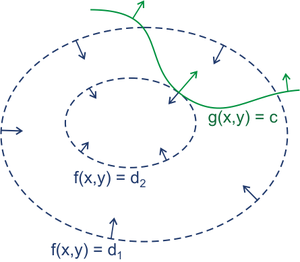
\includegraphics[scale = 0.5]{Lagrange_multiplier}\\
  \caption{Lagrange multiplier}\label{fig.Lagrange.multiplier}
\end{figure}

先看一个二维的例子:假设有函数:$f(x, y)$,要求其极值(最大值/最小值),且满足条件
$$ g\left( x,y \right) = 0, $$
c 为常数.对不同$d_n$的值,不难想像出

$$ f \left( x, y \right)=d_n $$
的等高线, 如图\ref{fig.Lagrange.multiplier},
\href{http://upload.wikimedia.org/wikipedia/commons/thumb/f/fa/Lagrange\_multiplier.png/300px-Lagrange\_multiplier.png}{Lagrange multiplier}所示.

假设g(x)与等高线相交,交点就是同时满足等式约束条件和目标函数的可行域的值,但肯定不是最优值,
因为相交意味着肯定还存在其它的等高线在该条等高线的内部或者外部,使得新的等高线与目标函数的交点的值更大或者更小,
只有到等高线与目标函数的曲线相切的时候,可能取得最优值(最大值或者最小值, 图中所示为最大值),
即等高线和目标函数的曲线在该点的法向量必须有相同方向,
所以最优值必须满足:f(x)的梯度 = a* g(x)的梯度,a是常数,表示左右两边同向.
这个等式就是L(a,x)对参数求导的结果

而方程 g 的可行集所构成的线正好是 $g ( x, y ) = c$ .想像我们沿着 $g = c$ 的可行集走,
因为大部分情况下 f 的等高线和 g 的可行集线不会重合,但在有解的情况下,这两条线会相交.想像此时我们移动 $g = c$ 上的点,因为 f 是连续的方程,
我们因此能走到$f \left( x, y \right)=d_n$更高或更低的等高线上,也就是说$d_n$可以变大或变小.只有当 $g = c$ 和$f \left( x, y \right)=d_n$相切,也就是说,
此时,我们正同时沿着 $g = c$ 和$f \left( x, y \right)=d_n$走.这种情况下,会出现极值或鞍点.

用向量的形式来表达的话,我们说相切的性质在此意味着 f 和 g 的切线在某点上平行.此时引入一个未知标量$\lambda$,并求解:

$$ \nabla \Big[f \left(x, y \right) + \lambda \left(g \left(x, y \right) - c \right) \Big] = 0 $$
且$\lambda \neq 0$.

一旦求出$\lambda$的值,将其套入下式,易求在无约束极值和极值所对应的点.

$$ F \left( x , y \right)  =  f \left( x , y \right) + \lambda \left( g \left( x , y \right) - c \right) $$
新方程$F(x,y)$在达到极值时与$f(x,y)$相等,因为$F(x,y)$达到极值时$g(x,y)-c$总等于零.

\subsection{Example}
\begin{example}
\textbf{求方程的最小值}:

$$ f(x, y) = x^2 y $$
同时未知数满足

$$ x^2 + y^2 = 1 $$
因为只有一个未知数的限制条件,我们只需要用一个乘数$\lambda$.

$$
\begin{aligned}
		& g (x, y) = x^2 +y^2 -1 \\
		& \Phi (x, y, \lambda) = f(x,y) + \lambda g(x, y) = x^2 y + \lambda (x^2 + y^2 - 1)
\end{aligned}
$$
将所有$\Phi$方程的偏微分设为零,得到一个方程组,最大值是以下方程组的解中的一个:

$$
\begin{aligned}
		& 2 x y + 2 \lambda x = 0 \\
		& x^2 + 2 \lambda y = 0 \\
		& x^2 + y^2 -1 = 0
\end{aligned}
$$
求解方程组,结果
\end{example}

\begin{example}
\textbf{离散分布的最大熵}:

$$ f(p_1,p_2,\ldots,p_n) = -\sum_{k=1}^n p_k\log_2 p_k.  $$
所有概率的总和是1,因此我们得到的约束是$g(p)= 1$即

$$ g(p_1,p_2,\ldots,p_n)=\sum_{k=1}^n p_k=1.  $$
可以使用拉格朗日乘数找到最高熵(概率的函数).对于所有的k 从1到n,要求

$$ \frac{\partial}{\partial p_k}(f+\lambda (g-1))=0, $$
由此得到

$$ \frac{\partial}{\partial p_k}\left(-\sum_{k=1}^n p_k \log_2 p_k + \lambda (\sum_{k=1}^n p_k - 1) \right) = 0.  $$
计算出这n个等式的微分,我们得到:

$$ -\left(\frac{1}{\ln 2}+\log_2 p_k \right) + \lambda = 0.  $$
这说明$p_i$都相等 (因为它们都只是$\lambda$的函数). 解出约束$\sum_k p_k = 1$,得到

$$ p_k = \frac{1}{n}.$$
因此,使用均匀分布可得到最大熵的值.
\end{example}

\section{KKT条件}
在满 足一些有规则的条件下,一个非线性规划(Nonlinear Programming)问题能有最优化解法的一个必要和充分条件.这是一个广义化拉格朗日乘数的成果.

考虑以下非线式最优化问题:
$$
\begin{aligned}
& \min\limits_{x}\;\; f(x) \\
& \mbox{Subject to: } g_i(x) \le 0 , h_j(x) = 0
\end{aligned}
$$
$f(x)$是需要最小化的函数,
$g_i (x)\ (i = 1, \ldots,m)$是不等式约束,
$h_j (x)\ (j = 1,\ldots,l)$是等式约束,
$m$和$l$分别为不等式约束和等式约束的数量.

把所有的不等式约束,等式约束和目标函数全部写为一个式子
$L(a, b, x)= f(x) + a*g(x)+b*h(x)$,
KKT条件是说最优值必须满足以下条件:

\begin{enumerate}
\item $L(a, b, x)$对x求导为零,
\item $h(x) =0$;
\item $a*g(x) = 0$;
\end{enumerate}
其中$a, h, g$都是向量表达形式

求取这三个等式之后就能得到候选最优值.其中第三个式子非常有趣, 因为
$g(x)<=0$,如果要满足第三个等式,必须$a=0$或者$g(x)=0$.\\
这是SVM的很多重要性质的来源,如支持向量的概念

而KKT条件是满足强对偶条件的优化问题的必要条件,可以这样理解:我们要求$min f(x), L(a, b, x) = f(x) + a*g(x) + b*h(x),a>=0$,
我们可以把$f(x)$写为:$max_{a,b} L(a,b,x)$,为什么呢?因为$h(x)=0, g(x)<=0$,现在是取$L(a,b,x)$的最大值,$a*g(x)<=0$,
所以$L(a,b,x)$只有在$a*g(x) = 0$的情况下才能取得最大值,否则,就不满足约束条件,
因此m$ax_{a,b} L(a,b,x)$在满足约束条件的情况下就是$f(x)$,因此我们的目标函数可以写为 $min_x max_{a,b} L(a,b,x)$.\\
如果用对偶表达式: $max_{a,b} min_x  L(a,b,x)$,由于我们的优化是满足强对偶的(强对偶就是说对偶式子的最优值是等于原问题的最优值的),
所以在取得最优值$x0$的条件下,它满足$f(x0) = max_{a,b} min_x  L(a,b,x) = min_x max_{a,b} L(a,b,x) =f(x0)$,我们来看看中间两个式子发生了什么事情:
$$ f(x0) = max_{a,b} min_x  L(a,b,x) =  max_{a,b} min_x f(x) + a*g(x) + b*h(x) =  max_{a,b} f(x0)+a*g(x0)+b*h(x0) = f(x0) $$

可以看到上述加黑的地方本质上是说 $min_x f(x) + a*g(x) + b*h(x)$ 在$x0$取得了最小值,用fermat定理,即是说对于函数 $f(x) + a*g(x) + b*h(x)$,求取导数要等于零,即

$$ f(x)的梯度+a*g(x)的梯度+ b*h(x)的梯度 = 0 $$

这就是kkt条件中第一个条件:$L(a, b, x)$对$x$求导为零.

而之前说明过,$a*g(x) = 0$,这时kkt条件的第3个条件,当然已知的条件$h(x)=0$必须被满足,
所有上述说明,满足强对偶条件的优化问题的最优值都必须满足KKT条件,即上述说明的三个条件.\\
可以把KKT条件视为是拉格朗日乘子法的泛化.
\end{document}
